Debido a la \textit{"intratabilidad"} del problema de la partición de grafos, como hemos comentado, no existe un algoritmo concreto que permita obtener en tiempo polinómico una solución óptima a la partición de cualquier grafo. Es por ello por lo que, los algoritmos codificados para este informe se basan en la metaheurística, con el objetivo de obtener soluciones de buena calidad en tiempos computacionales aceptables, a pesar de que los algoritmos metaheurísticos no garantizan que se vaya a obtener una solución óptima al problema.

En el siguiente apartado se describen los algoritmos Kernighan-Lin\cite{KernighanLin} (ver apartado \ref{Kernighan-Lin}), Specrtal Bisection (ver apartado \ref{Spectral-Bisection}) y Multilevel Spectral Bisection (ver apartado \ref{Multilevel-Spectral-Bisection}). Tres algoritmos que se diseñaron específicamente para la resolución del problema de la partición de grafos. Cualquiera de estos algoritmos proporciona una solución factible al problema, pudiendo ser esta óptima o no. El enfoque del informe radica en la partición de diferentes grafos en dos particiones usando estos tres algoritmos. 

Además de describir cada uno de los algoritmos, también se describirán algunos detalles sobre su codificación.
De ejemplo para describir cada codificación se ha utilizado un grafo inicial (ver Figura \ref{grafo}). Este grafo es un grafo no dirigido (ver Definición \ref{no_dirigido}) de diez nodos con pesos en sus aristas.

\begin{mydef}\label{no_dirigido}
	Un grafo no dirigido es un grafo (ver Definición \ref{def:grafo} ) donde: $V\neq \emptyset$ y $E\subseteq \{x\in \mathcal P(V):|x|=2\}$ es un conjunto de pares no ordenados de elementos de $V$. Un par no ordenado es un conjunto de la forma \{a , b\}, de manera que \{a, b\} = \{b, a\}. En los grafos, los subconjuntos de pares no ordenados pertenecen al conjunto potencial de $V$, denotado $\mathcal P(V)$, y son de cardinalidad 2. 
\end{mydef}

\renewcommand{\figurename}{Figura}
\begin{figure}[h]
	\centering
	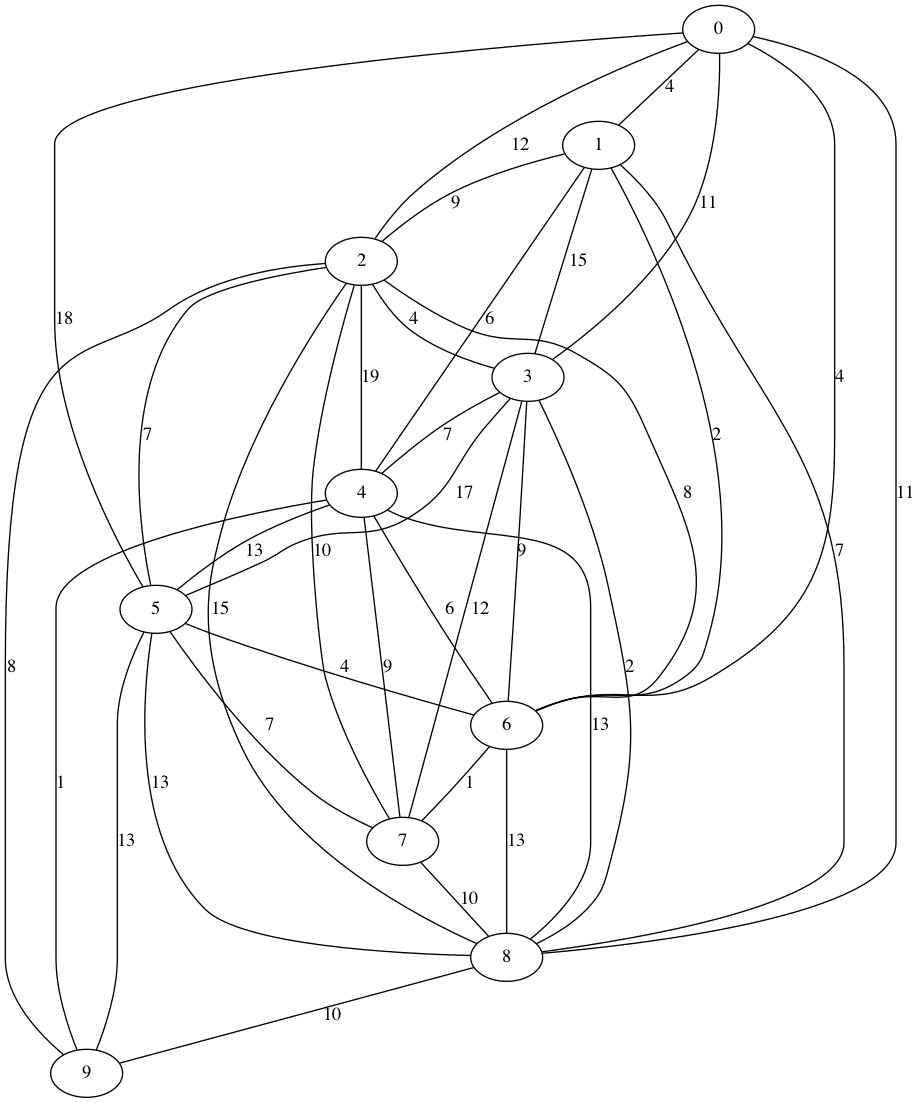
\includegraphics[scale=0.25]{Figures/10_dataset}
	\vspace{1mm}
	\caption{Grafo inicial.}
	\label{grafo}
\end{figure}

\newpage
\section{Kernighan-Lin}\label{Kernighan-Lin}

El algoritmo Kernighan-Lin\cite{KernighanLin}, a menudo abreviado como K-L, es uno de los primeros algoritmos de partición de grafos y fue desarrollado originalmente para optimizar la colocación de circuitos electrónicos en tarjetas de circuito impreso para minimizar el número de conexiones entre las tarjetas (circuitos VLSI\cite{KernighanLin}\cite{Ravikumar}).

El algoritmo es:

\begin{itemize}
	\setlength{\parskip}{0pt}
	\setlength{\itemsep}{0pt plus 1pt}
	\item \textbf{Iterativo}. Porque el grafo inicialmente ya está particionado, pero la aplicación del algoritmo intentará mejorar u optimizar la partición inicial. 
	\item \textbf{Voraz}. Porque el algoritmo hará cambios si hay un beneficio inmediato sin considerar otras formas posibles de obtener una solución óptima. Para ello, elige la opción óptima en cada paso con la esperanza de llegar a una solución general óptima.
	\item \textbf{Determinista}. Porque se obtendrá el mismo resultado cada vez que se aplique el algoritmo. 
\end{itemize}

El algoritmo K-L, como acabamos de describir, no crea particiones, sino que las mejora iterativamente. La idea original era tomar una partición aleatoria y aplicarle Kernighan-Lin\cite{KernighanLin}. Esto se repetiría varias veces y se elegiría el mejor resultado. Mientras que para grafos pequeños esto ofrece resultados razonables, es bastante ineficiente para tamaños de grafos más grandes.

Hoy en día, el algoritmo se usa para mejorar las particiones encontradas por otros algoritmos, tratando de mejorar las particiones mediante el intercambio de nodos vecinos. Por tanto, complementa muy bien otro tipo de algoritmos como por ejemplo los que realizan una partición espectral (ver sección \ref{Spectral-Bisection}).

\subsection{Descripción}

El objetivo del algoritmo es dividir el conjunto de vértices $V$ de un grafo no dirigido (ver Definición \ref{no_dirigido}) en dos subconjuntos disjuntos (ver Definición \ref{disjuntos}) $A$ y $B$ de igual tamaño, de una manera que minimice la suma $T$ de los pesos del subconjunto de aristas que cruzan de $A$ a $B$. El algoritmo mantiene y mejora una partición, en cada iteración usando un algoritmo voraz (ver Definición \ref{voraz}), empareja los vértices de $A$ con los vértices de $B$, de modo que al mover los vértices emparejados de una partición a la otra se maximiza la ganancia, que mide cuánta "información" nos brinda la función objetivo. Después de emparejar los vértices y maximizar la ganancia, crea un subconjunto de los pares de los vértices elegidos para tener el mejor efecto sobre la calidad de la solución $T$. Dado un grafo con n vértices, cada iteración del algoritmo se ejecuta en el tiempo $O({n}^2 \, log \, n)$.

\begin{mydef}\label{disjuntos}
	$A$ y $B$ son dos subconjuntos disjuntos si $A \cup B$ y $A \cap B \neq 0$.
\end{mydef}

\begin{mydef}\label{voraz}
	Dado un conjunto finito $C$, un algoritmo voraz devuelve un conjunto $S$ tal que $S\subseteq C$ y que además cumple con las restricciones del problema inicial. A cada conjunto $S$ que satisfaga las restricciones y que logra que la función objetivo se minimice o maximice (según corresponda) diremos que $S$ es una solución óptima. 
\end{mydef}

Más detalladamente, sea $a$ un elemento del subconjunto $A$ y $b$ un elemento del subconjunto $B$, para cada $a \in A$, $I_{a}$ es el coste interno de a, es decir, la suma de los pesos de las aristas entre a y otros nodos en $A$. Y $E_{a}$ es el coste externo de a, es decir, la suma de los pesos de las aristas entre a y los nodos en $B$. De manera similar, se define $I_{b}$ y $E_{b}$ para cada $b \in B$.

Así podemos decir que existe una diferencia $D$ entre la suma de los costes externos e internos $s$. Si formalizamos obtenemos:

\begin{center}
	$D_{s} = E_{s} - I_{s}$
\end{center}

Y entonces si $a$ y $b$ se intercambian, la ganancia se calcula como:

\begin{center}\label{ganancia}
	$T_{antigua} - T_{nueva} = D_{a} + D_{b} - 2c_{a, b}$ 
\end{center}

donde $c_{a, b}$ es el coste de las aristas posibles entre $a$ y $b$.

El algoritmo intenta encontrar una solución óptima de operaciones de intercambio entre los elementos de $A$ y $B$ que maximice la ganancia ($T_{antigua} - T_{nueva}$) y luego ejecuta las operaciones, produciendo una partición del grafo en $A$ y $B$.

Con estos dos conceptos, podemos describir la primera iteración del algoritmo usando el pseudocódigo en \cite{Ravikumar}.

\begin{figure}[h]
	\centering
	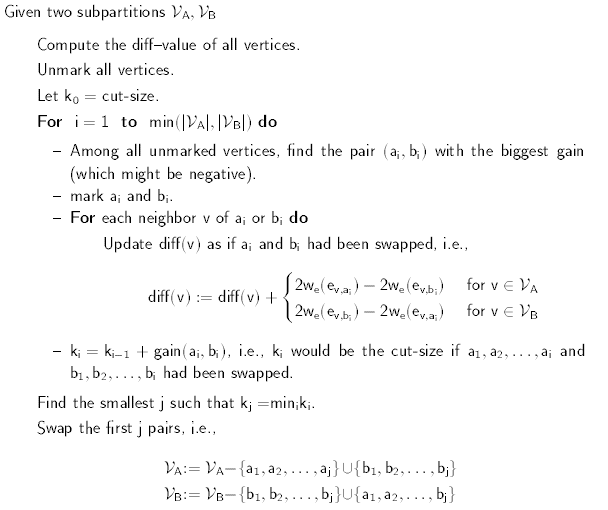
\includegraphics[scale=0.8]{Figures/kl_pseudocode}
	\vspace{1mm}
	\caption{Kernighan-Lin.}
	\label{kl_pseudocode}
\end{figure}

Entonces, en cada iteración, el algoritmo K-L intercambia pares de vértices para maximizar la ganancia. Y continúa haciéndolo hasta que se intercambian todos los vértices de la partición más pequeña. 

C. Fiduccia y R. Mattheyses realizaron importantes avances prácticos en \cite{FiducciaMattheyses}, quienes mejoraron el algoritmo de  Kernighan-Lin\cite{KernighanLin} de tal manera que, cada partición se ejecuta en $O({n}^2)$, en lugar de $O({n}^2 \, log \, n)$. La reducción se logra en parte eligiendo nodos individuales para intercambiar en lugar de parejas de vértices.

Una gran ventaja del algoritmo es que no se detiene incluso aceptando ganancias negativas, sigue esperando que las ganancias posteriores sean más grandes y que el tamaño de la suma de los pesos de las aristas se reduzca hasta que se intercambian todos los vértices de la partición más pequeña. 

Esta capacidad es una característica crucial. Aunque esta capacidad sea crucial, el algoritmo tiene unas cuantas desventajas.

Podemos decir que las principales desventajas son:

\begin{itemize}
	\item Los resultados son aleatorios porque el algoritmo comienza con una partición aleatoria.
	\item Computacionalmente es un algoritmo lento.
	\item Solo se crean dos particiones del mismo tamaño.
	\item Las particiones deben tener el mismo tamaño para que el algoritmo no intente encontrar soluciones óptimas que ya existan.
	\item No resuelve muy bien los problemas con las aristas ponderadas.
	\item La solución dependerá en gran medida de la primera partición.
\end{itemize}

\subsection{Ejemplo de codificación}\label{Kernighan-Lin-ejemplo}

Existen muchas variaciones del algoritmo K-L que a menudo intercambian el tiempo de ejecución con la calidad, o generalizan el algoritmo a más de dos particiones. En este caso, para la codificación del algoritmo se ha utilizado la libraría de Python: \href{https://networkx.github.io/documentation/stable/reference/algorithms/generated/networkx.algorithms.community.kernighan_lin.kernighan_lin_bisection.html}{NetworkX}. El algoritmo divide un grafo en dos particiones usando el algoritmo Kernighan-Lin\cite{KernighanLin}. Es decir, divide un grafo en dos subconjuntos intercambiando iterativamente pares de nodos para reducir el peso de las aristas entre los dos subconjuntos.

\begin{mydef}\label{NetworkX}
	NetworkX es un paquete de Python para la creación, manipulación y estudio de la estructura, dinámica y funciones de los grafos. 
\end{mydef}

Por ejemplo, en una ejecución de la codificación, donde la entrada es el grafo de la Figura \ref{grafo}, y después de una partición inicial, podemos obtener los subconjuntos: A = \{3, 4, 6, 8, 9\} y B = \{0, 1, 2 , 5, 7\}. Estos subconjuntos son del mismo tamaño y sus elementos están ordenados.

En esta ejecución, los pasos que sigue el algoritmo son los siguientes:

\begin{itemize}
	\item Dibuja una línea que separa el grafo en dos particiones con el mismo número de vértices en cada partición.
	\item Cuenta la cantidad de aristas que cruzan la línea. Este número se llama \textit{"cut-size"} y el objetivo es disminuirlo, es decir, disminuir el número de conexiones entre los vértices del grafo.
	\item Encuentra el coste de todos los vértices en el grafo, buscando el número de conexiones que cada vértice tiene dentro de su propia partición y restando eso del número de conexiones que cada vértice tiene con vértices en la otra partición.
	\item Determina la ganancia máxima intercambiando dos nodos. La ecuación de ganancia es la que se muestra en \ref{ganancia}.
	\item Intercambia los dos nodos con la ganancia máxima. Si se han calculado todas las ganancias de emparejamiento de todos los nodos y la ganancia máxima es igual a cero o negativa, los nodos con la ganancia más alta aún deberán intercambiarse.
	\item Resta la ganancia del \textit{"cut-size"} original para obtener el nuevo \textit{"cut-size"}.
	\item Cambia los nodos que se han intercambiado.
	\item Repite estos pasos hasta que la ganancia máxima es cero o negativa.
\end{itemize}

\newpage
Los pasos que sigue el algoritmo que acabamos de describir se pueden visualizar en la siguiente figura,

\begin{figure}[h]
	\centering
	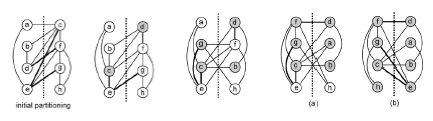
\includegraphics[scale=0.9]{Figures/KL_steps}
	\vspace{1mm}
	\caption{Kernighan-Lin.}
	\label{KL_steps}
\end{figure}

\section{Spectral Bisection}\label{Spectral-Bisection}

El algoritmo de bisección espectral que se describe en la siguiente sección es bastante diferente al algoritmo que acabamos de describir. Ya que no utiliza el grafo en sí, sino una representación matemática del mismo, una matriz.

\subsection{Descripción}

El método de bisección espectral aborda el problema de la partición de grafos con un estrategia desarrollada por Pothen, Simon y Liou\cite{PothenSimon}. El método se basa en el cálculo del \textit{eigenvector}, denominado vector de Fiedler\cite{Fiedler}, correspondiente al segundo \textit{eigenvalue} más pequeño de la matriz laplaciana $L(G = A_{i,j})$ del grafo $G$ que se define:

\begin{center}
	$$
	A_{ij} = 
	\begin{cases}
	-1 & \text{if $i \neq j \, and \, e_{i, j} \in E$} \\
	0 & \text{if $i \neq j \, and \, e_{i, j} \notin E$} \\
	 deg(v_{i}) & \text{if i = j} 
	\end{cases}
	$$
\end{center}

Se ve fácilmente que la matriz laplaciana se define como $L(G) = D - A$, donde $A$ es la matriz de adyacencia (ver Definición \ref{matriz_adyacencia}) del grafo y D es la diagonal de la matriz que representa el \textit{eigenvector} para cada \textit{eigenvalue} del grafo. En el caso de que el grafo tenga pesos en las aristas, $W_{e}$, el grafo $G$ se definiría:

\begin{center}
	$$
	A_{ij} = 
	\begin{cases}
	-W_{e}(e_{i, j}) & \text{if $i \neq j \, and \, e_{i, j} \in E$} \\
	0 & \text{if $i \neq j \, and \, e_{i, j} \notin E$} \\
	\sum_{k=1}^{n} W_{e}(e_{i, j}) & \text{if i = j} 
	\end{cases}
	$$
\end{center}

El principal objetivo del algoritmo de bisección espectral, como acabamos de comentar, es el cálculo del vector de Fiedler\cite{Fiedler}, además de minimizar el coste del número de aristas del grafo. En tal escenario, el \textit{eigenvalue} más pequeño ($\lambda_{2}$) de $L$ produce un coste óptimo (c) tal que $c \geqslant \frac{\lambda_{2}}{n}$, donde $n$ es le número de nodos del grafo. Así, el \textit{eigenvector} que corresponde a $\lambda_{2}$ es el vector que se denomina vector de Fiedler. 

En general, esto produce una buena partición (pero no necesariamente la mejor). La partición obtenida por el segundo \textit{eigenvalue} puede ser potencialmente mejorada tratando de maximizar el \textit{eigenvalue} mínimo de la matriz $L$ al encontrar un cambio apropiado en los elementos de la diagonal $D$. Sin embargo, esta técnica requiere el cálculo de todos los \textit{eigenvalues} de la matriz laplaciana $L$. Esto no es muy factible computacionalmente para los grafos con muchos nodos.

La implementación original de este algoritmo utiliza el algoritmo de Lanczos (ver Definición \ref{Lanczos}) modificado para calcular los vectores de Fiedler\cite{Fiedler}. 

\begin{mydef}\label{Lanczos}
	El algoritmo de Lanczos es un algoritmo iterativo creado por Cornelius Lanczos\cite{Lanczos}, que es una adaptación de los métodos iterativos para encontrar los \textit{eigenvalues} más útiles y el \textit{eigenvector} de una matriz de dimensión $N x N$ realizando un número de operaciones $M$, donde el valor de $M$ será más pequeño que $N$. 
\end{mydef}

Para dividir un grafo en un número de particiones de potencia de dos, el algoritmo de bisección espectral aplica los siguientes pasos:

\begin{enumerate}
	\item Calcula el vector de Fiedler utilizando el algoritmo Lanczos sin factorizar.
	\item Ordena los vértices de acuerdo con los tamaños de los componentes del vector Fiedler.
	\item Asigna la mitad de los vértices a cada subpartición.
	\item Aplica los pasos 1-3 a cada subpartición hasta obtener el número deseado de particiones.
\end{enumerate}

La principal etapa de este algoritmo es el primer paso, el cálculo del vector de Fiedler. Y nos da una idea de cómo funciona el algoritmo. A contaminación, mostraremos su pseudocódigo y luego se intenta explicar cómo funciona en la siguiente sección.

\begin{figure}[h]
	\centering
	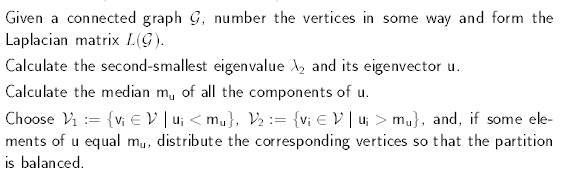
\includegraphics[scale=0.8]{Figures/bisection_pseudocode}
	\vspace{1mm}
	\caption{Spectral Bisection.}
	\label{bisection_pseudocode}
\end{figure}

\subsection{Ejemplo de codificación}

La partición de grafos usando un método de partición espectral se basa álgebra lineal. Sin embargo, los métodos espectrales para la partición de grafos son algoritmos computacionalmente caros. El algoritmo utilizado en la codificación calcula la matriz laplaciana $L$ del grafo de entrada inicial (ver Figura \ref{grafo}). Pero antes de describir la codificación introduciremos los conceptos de matriz de adyacencia (ver Definición \ref{adyacencia}) y matriz laplaciana (ver Definición \ref{laplaciana}), ya nombrados anteriormente en la sección anterior.

\begin{mydef}\label{adyacencia}
	Una propiedad importante de los nodos de un grafo es su grado. El grado de un nodo es el número de aristas que están conectadas a él. Si para dos nodos A y B hay una arista uniéndolos, decimos que A y B son adyacentes. Así, se puede describir un grafo en una matriz de adyacencia. Esta es una matriz en la que se describe la conectividad de todos los nodos en el grafo. Una matriz de adyacencia A de un grafo G con N nodos es una matriz con el tamaño de N x N. La posición dentro de la matriz $A_{ij}$ representa la conectividad del nodo j con el nodo i. Si hay una arista entre el nodo j y el nodo i, entonces el valor en la posición de matriz $A_{ij}$ será uno, en todos los demás casos será cero. 
	\newpage
	Esto se puede describir como tal:
	\begin{center}
		$$
		A_{ij} = 
		\begin{cases}
			\text{1 si hay una arista que va del nodo j el nodo i} \\
			\text{0 otros casos}
		\end{cases}
		$$
	\end{center}
	En un grafo no dirigido (el caso estudiado en este informe), el valor en la posición en la matriz de adyacencia de $A_{ij}$ será el mismo que el valor en la posición $A_{ij}$. Ver ejemplo de una matriz de adyacencia en la Figura \ref{matriz_adyacencia}.
\end{mydef}

\begin{mydef}\label{laplaciana}
	La matriz de grados es una matriz que se puede construir a partir de la matriz de adyacencia (ver Definición \ref{adyacencia}). Esto se puede hacer construyendo un vector de grado de 1 x N, como ejemplo podemos verlo en la Figura \ref{matriz_adyacencia}. Este vector contiene en el elemento i la suma de la fila del número de columna j de la matriz de adyacencia. La matriz de grados se construye multiplicando el vector de grados con la matriz de identidad de tamaño N x N. Con la matriz de grados D y la matriz de adyacencia A, se puede construir la matriz laplaciana L. Esto se puede hacer restando A de D.
	\begin{center}
		$L_{ij} = D_{ij} - A_{ij}$
	\end{center}
	La matriz laplaciana se puede definir mediante el siguiente conjunto de reglas:
	\begin{center}
		$$
		A_{ij} = 
		\begin{cases}
		k(i), & \text{if i = j} \\
		-1, & \text{if $\exists$ e(i,j)} \\
		0, & \text{otros casos}
		\end{cases}
		$$
	\end{center}
	La matriz laplaciana tiene la entrada -1 donde la matriz de adyacencia tiene un valor distinto de cero. Los grados se representan en diagonal. Todos los demás valores son cero.
\end{mydef}

A continuación, describimos como se obtienen los denominados \textit{eigenvalues} y \textit{eigenvectors} de la matriz laplaciana. Se obtienen mediante álgebra lineal directa. Los \textit{eigenvalues} (y sus \textit{eigenvectors} correspondientes) se ordenan en función de la magnitud: $\lambda_{0} = 0 \leq \lambda_{1} \leq \lambda_{n-1}$. El eigenvector correspondiente al \textit{eigenvalue} más pequeño consiste exclusivamente de unos. Este vector no tiene ningún uso práctico ya que no se puede recuperar información útil de él. Sin embargo, el segundo eigenvector más pequeño contiene la información necesitaba para hacer la partición espectral. Este vector también se conoce como el vector de Fiedler\cite{Fiedler} y se define formalmente:

\begin{center}
	$v^{-T} \cdot L(G) \cdot \vec{v} = \sum_{i,j \in E}^{} (x_{i} - x_{j})^2$
\end{center}

\begin{center}
	$\lambda_{1} = \frac{min}{\vec{v} \perp (1, ..., 1)} \left(\frac{v^{-T} \cdot L(G) \cdot \vec{v}}{v^{-T} \cdot \vec{v}} \right)$
\end{center}

Cuando se calcula el \textit{eigenvalue} correspondiente del vector de Fiedler de la matriz laplaciana, se puede ver si el grafo está conectado o no. Este número también se conoce como la conectividad algebraica [6]. Esto es útil ya que la partición espectral solo puede ser efectiva si el grafo está conectado. Esto se debe a que la partición espectral se centra en minimizar el peso de las aristas. En un gráfico desconectado, esto sería cero. 

\newpage
Una vez que se encuentra el vector de Fiedler, se calcula el valor medio:

\begin{center}
	$Pivote = \frac{\sum (\text{componentes de Fiedler})}{\text{Número de componentes}}$
\end{center}

Con este pivote, los nodos que se corresponden con los \textit{eigenvalues} se pueden dividir en dos partes. Todos los nodos con los \textit{eigenvalues} correspondientes debajo del pivote se particionan en la partición A y todos los demás nodos se colocarán en la partición B. Este método se ha utilizado para la codificación del algoritmo de partición espectral. Que después de ejecutar un partición de ejemplo podemos obtener los subconjuntos: A = \{1, 2, 3, 4, 6, 9\} y B = \{0, 8, 5, 7\}. En este caso, los subconjuntos no son del mismo tamaño, y tampoco se encuentran ordenados. Es una de las diferencias más significativas entre las codificaciones de Kernighan-Lin y Multilevel Spectral Bisection con esta codificación (Spectral Bisection). El algoritmo de partición espectral se llama de forma recursiva para crear las dos particiones. Esto indica que el número de particiones se ha limitado expresamente a dos. Sin embargo, el algoritmo no es perfecto, como vemos, no crea particiones perfectamente equilibradas (con el mismo número de nodos).

\begin{figure}[h]
	\centering
	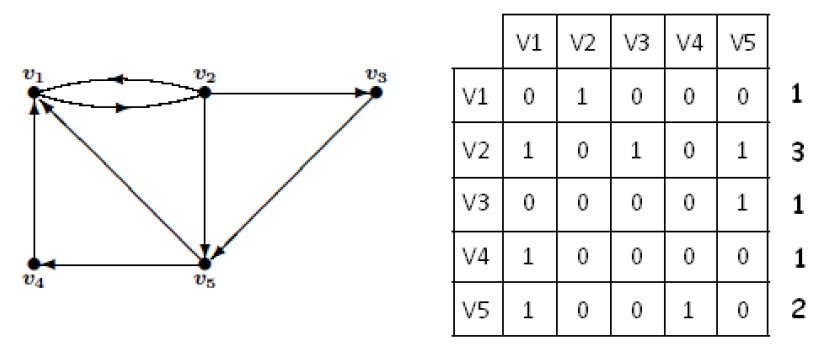
\includegraphics[scale=0.45]{Figures/matriz}
	\vspace{1mm}
	\caption{Matriz de adyacencia.}
	\label{matriz_adyacencia}
\end{figure}

\section{Multilevel Spectral Bisection}\label{Multilevel-Spectral-Bisection}

El particionamiento de grafos por \textit{multilevel} es un método moderno, que reduce el tamaño de las particiones del grafo con la combinación de los vértices y las aristas sobre varios niveles, creando particiones del grafo cada vez más pequeñas y extensas, con muchas variaciones y combinaciones de diferentes métodos. Tampoco utiliza el grafo en sí, sino una representación matemática del mismo, una matriz. La técnica \textit{multilevel} calcula el vector de Fiedler\cite{Fiedler} mucho más eficientemente.

\subsection{Descripción}\label{msb_description}

Al algoritmo de bisección espectral multinivel se basa en la construcción sucesiva de una serie de pequeñas matrices, cada una de las cuales se aproxima a su predecesora más grande. En algún momento, la matriz es tan pequeña que el algoritmo de Lanczos\cite{Lanczos} puede calcular el vector Fiedler\cite{Fiedler} de la matriz laplaciana en un período de tiempo insignificante. Este vector se interpola en el siguiente nivel superior, produciendo una aproximación de alto grado en el vector Fiedler para la matriz laplaciana correspondiente a este nivel. El vector intercambiado es entonces mejorado usando el algoritmo de iteración del cociente de Rayleigh (ver Definición \ref{Rayleigh}). El proceso continúa hasta que se obtiene el vector de Fiedler para la matriz original.

\begin{mydef}\label{Rayleigh}
	En matemáticas, dado una matriz $M$ y un vector distinto de cero $x$, el cociente de Rayleigh , se define como $R(M, x)$, tal que:
	\begin{center}
		$R(M, x)$ = $\frac{x \cdot Mx}{x \cdot x}$
	\end{center}
\end{mydef}


La idea de la técnica de multinivel es la de reducir la magnitud de un grafo, calcular una partición en este grafo reducido, y finalmente proyectar esta partición en el grafo original. Dado un grafo inicial, intentamos reducirlo con un nuevo grafo que en cierto sentido es similar, pero con menos vértices, más pequeño. Ya que el nuevo grafo es más pequeño, es más barato calcular el vector de Fiedler del nuevo grafo.

El cálculo del vector de Fiedler propio para MSB sería así:

\begin{figure}[h]
	\centering
	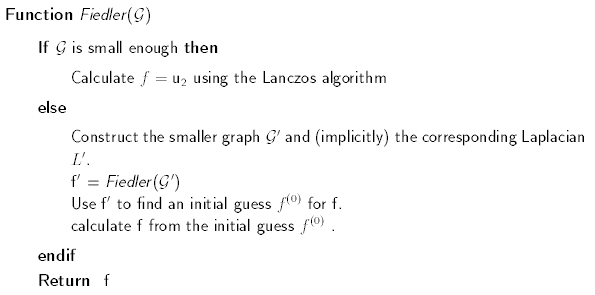
\includegraphics[scale=0.8]{Figures/fiedler}
	\vspace{1mm}
	\caption{Cálculo del vector de Fiedler para MSB.}
	\label{fiedler}
\end{figure}

Por supuesto, se han omitido tres detalles bastante importantes: cómo construir el grafo más pequeño (fase de contracción), cómo encontrar una función inicial $f^(0)$ para $f$ (fase de intercalación) y cómo calcular eficientemente $f$ usando $f^(0)$ (fase de refinamiento). El algoritmo requiere que se agreguen estos tres elementos al nivel único básico del algoritmo de bisección espectral.

\begin{itemize}
	\item \textbf{Contracción}. La construcción de una serie de grafos más pequeños, que conserven la estructura del grafo original. En esta primera fase el grafo se reduce mediante la fusión de sus vértices. La fusión de los vértices se realiza de forma iterativa: de un grafo se crea un nuevo grafo más grande y de este nuevo grafo más grande se crea un grafo aún más grande. Esto se hace hasta que una pequeña cierta magnitud es alcanzada. De este modo se crean grafos con diferentes magnitudes. 
	\item \textbf{Intercalación}. Dado un vector de Fiedler de un grafo más pequeño que el original, intercalar este vector al siguiente grafo más grande de manera que proporcione una buena aproximación al siguiente vector de Fiedler. Así se crea una partición del grafo más grande con la magnitud más pequeña. 
	\item \textbf{Refinamiento}. La partición calculada iterativamente se proyecta de nuevo al grafo original. En cada iteración se aplica un refinamiento usando el algoritmo del cociente de Rayleigh. El refinamiento se usa para asegurar que el cálculo más preciso de manera eficiente del vector de Fiedler. En este proceso se usa el algoritmo del cociente de Rayleigh (ver Figura) dado el el vector de Fiedler de un grafo aproximado. 
\end{itemize}

\begin{figure}[h]
	\centering
	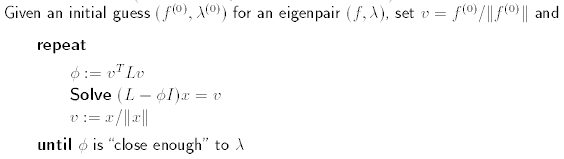
\includegraphics[scale=0.8]{Figures/rayleigh}
	\vspace{1mm}
	\caption{Iteración del cociente de Rayleigh.}
	\label{rayleigh}
\end{figure}

Con estas mejoras respecto al algoritmo de bisección espectral, La técnica multinivel mejorará significativamente los resultados, tanto en términos de calidad y tiempo de funcionamiento.

\newpage
\subsection{Ejemplo de codificación}

Para la codificación del algoritmo MSB se ha usado uno de los algoritmos más exitosos para el problema de partición de grafos, el algoritmo METIS. METIS\cite{MeTis} es un algoritmo que se enfoca en minimizar el número de aristas cruzadas de cada partición y distribuir el número de nodos de manera uniforme entre las particiones. La Figura \ref{metis} muestra el algoritmo:

\begin{figure}[h]
	\centering
	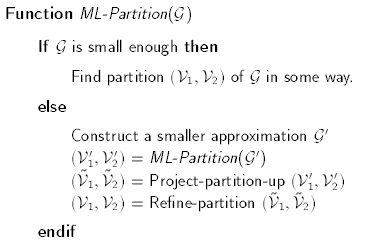
\includegraphics[scale=0.8]{Figures/metis}
	\vspace{1mm}
	\caption{Algoritmo METIS.}
	\label{metis}
\end{figure}

Como algoritmo MSB, con METIS, los grafos se dividen en tres fases (ver sección \ref{msb_description}). La primera fase es la fase de engrosamiento, la segunda la fase de partición y la tercera y última fase la fase de no engrosamiento (ver Figura \ref{metis}). A continuación, se muestra una breve explicación de estas fases dentro del algoritmo METIS.

\textbf{La fase de engrosamiento}. El objetivo principal de la fase de engrosamiento dentro del algoritmo METIS es reducir el grafo original a un grafo más pequeño, que aún contiene suficiente información para hacer una buena partición. Esto sucede con el uso de un algoritmo de coincidencia. Hay varios algoritmos de coincidencia, los más destacados son el algoritmo de coincidencia pesada y el algoritmo de coincidencia aleatoria. El algoritmo de coincidencia pesada inicialmente coincide con los pesos de las aristas más pesados. En cambio, el algoritmo de coincidencia aleatoria selecciona aleatoriamente los vértices más conectados (con más conexiones entre dos vértices). 

\textbf{La fase de partición}. El objetivo principal de la fase de partición dentro del algoritmo METIS es dividir el grafo en dos partes balanceadas mientras se minimiza el número de conexiones entre los vértices. En esta fase se utilizan algoritmos de partición de grafos para una bisección inicial, como Spectral Bisection (ver sección \ref{Spectral-Bisection}), Kernighan-Lin (ver sección \ref{Kernighan-Lin}), etc.  

\textbf{La fase de no engrosamiento}. El objetivo principal de la fase de no engrosamiento (descomposición) dentro del algoritmo METIS es el reajuste de las particiones creadas por el algoritmo de partición. Este proceso se realizará varias veces donde se aplicará un algoritmo de refinamiento para garantizar un buen equilibrio en cada partición.

\begin{figure}[h]
	\centering
	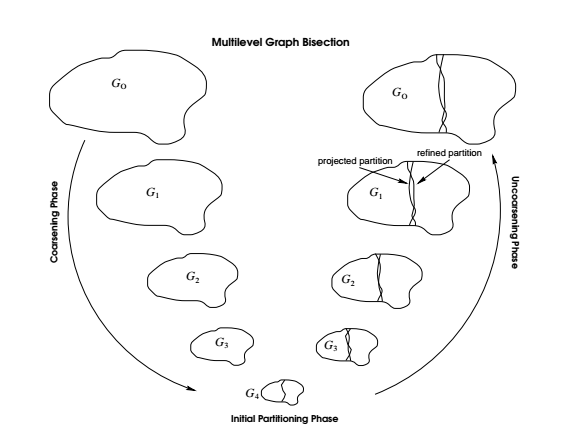
\includegraphics[scale=0.7]{Figures/fases}
	\vspace{1mm}
	\caption{Fases de MSB.}
	\label{fases}
\end{figure}

\newpage
Las características clave del algoritmo son las siguientes:

\begin{itemize}
	\item Proporciona particiones de alta calidad. Los experimentos con una gran cantidad de nodos muestran que METIS produce particiones que son consistentemente mejores que las producidas por otros algoritmos ampliamente utilizados. Las particiones producidas por el algoritmo METIS son consistentemente de un 10\% a un 50\% mejores que las producidas por algoritmos de partición espectral.
	\item Es extremadamente rápido. Los experimentos en una amplia gama de grafos han demostrado que el algoritmo METIS es de uno a dos órdenes de magnitud más rápido que otros algoritmos de partición ampliamente utilizados.
\end{itemize}

Para la codificación del algoritmo en este informe se escogió la librería de Python: \href{https://networkx-metis.readthedocs.io/en/latest/reference/generated/nxmetis.partition.html#nxmetis.partition}{NetworkX-METIS}. \textit{NetworkX-METIS} es un complemento para la libraría de \textit{NetworkX} que usa el algoritmo METIS para la partición de grafos. Por ejemplo, en una ejecución de la codificación, donde la entrada es el grafo de la Figura \ref{grafo}, se han creado los subconjuntos: A = \{0, 1, 3, 7, 8\} y B = \{2, 4, 5, 6, 9\}. Estos subconjuntos tienen el mismo tamaño y sus elementos están ordenados, igual que en la sección \ref{Kernighan-Lin-ejemplo}. El algoritmo ha resultado ser muy eficiente (ver sección \ref{chapter:Comparativa}).